\documentclass[a4paper,11pt,titlepage]{article}

\newcommand{\MEM}{Moorman}
\newcommand{\KM}{May}
\newcommand{\SK}{Kress}
\newcommand{\MM}{Marin}
\newcommand{\JN}{Nanda}
%shortcuts
\newcommand{\ra}{
  $\rightarrow$ \xspace
}
\usepackage{vhistory}
\usepackage{graphicx}
\usepackage{enumerate}
\usepackage{xspace}
\usepackage{amsmath}
\usepackage{import}
\usepackage{expdlist}
\usepackage{float}
% title definition
\author{Team G2 \\
        Seth Kress\\ 
        Kenny May\\ 
        Michael Moorman\\
        Jagriti Nanda\\
        Misael Marin}
\title{DARS Use Cases (v\vhCurrentVersion)}

\date{\today}

\begin{document}

%generate the title page
\maketitle


%generate the table of contents
\tableofcontents

\newpage

\begin{versionhistory}
% Note the syntax of \vhEntry! Authors are separated by `|'         %%
\vhEntry{1.0}{2010-10-14}{\MEM|\KM|\SK|\MM|\JN}{Initial version.}            %%
\end{versionhistory}

\newpage

\section{Introduction}
This document's primary purpose is to identify and elaborate upon all of the use cases exposed by the Dynamic Ad-Hoc Routing Simulator (DARS). Furthermore, three main usage scenarios are presented. These scenarios tie together use cases in a narrative format.

\section{Overview}
The following table lists all of the use cases specified in this document. \\
\begin{center}
\begin{tabular}{ | c | c | }
  \hline
  {\bf{Use Case}} & {\bf{Use Case ID}} \\
  \hline
  Create New Simulation & UC-A \\
  \hline
  Configure Network Node & UC-B \\
  \hline
  Change Simulation Speed & UC-C \\
  \hline
  Start Simulation & UC-D \\
  \hline
  Pause Simulation & UC-E \\
  \hline
  Resume Simulation & UC-F \\
  \hline
  Send Message & UC-G \\
  \hline
  View Node Information & UC-H \\
  \hline
  End Simulation & UC-I \\
  \hline
  Save Log & UC-J \\
  \hline
  Load Replay File & UC-K \\
  \hline
  Load Simulation Setup & UC-L \\
  \hline
\end{tabular}
\end{center}
\section{Usage Scenarios}

\subsection{Manual Mode (Typical) Scenario}
The manual mode scenario represents the course of events that a typical user would take when using DARS. 
 
Here, the DARS graphical interface is used to manually configure and arrange the nodes of the simulated network. After configuring this and the simulation speed, the user begins the simulation. The user continues to interact while the simulation runs. They can add, remove, or edit network nodes as the simulation unfolds. They may also send a message from one network node to another and view the behavior in real time.
 
At any time during the simulation, the user may pause the simulation. From there, they can then change network nodes, simulation speed, or en-queue a message to be sent from one node to another. The simulation is resumed later by a user action.
 
The user concludes the simulation at any time after the simulation has begun. After this action, the user may optionally save the simulation results and input data into a log file. 
The manual mode or typical scenario exposes the use cases shown in figure \ref{fig:scen1} below.

\begin{figure}[H]
        \centering
	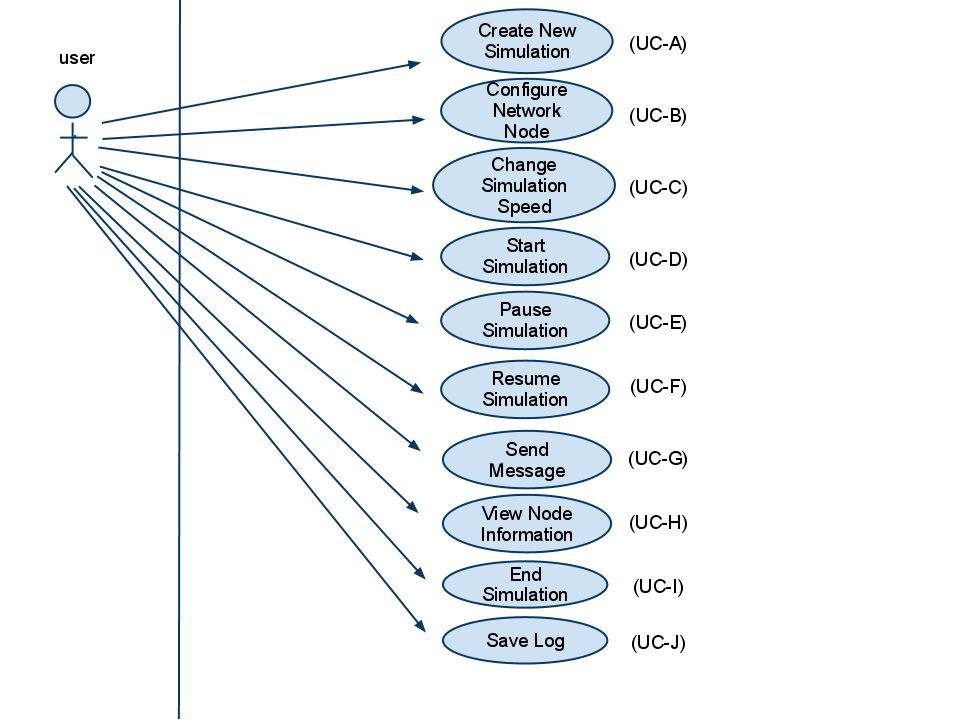
\includegraphics[height=150mm]{img/scenario1.png}
        \caption{Usage Scenario 1: Manual Mode}
        \label{fig:scen1}
\end{figure}

\subsection{Batch Mode Scenario}
The batch mode scenario represents the course of events that a user would take when replaying a simulation run that was already created. DARS consumes a log file that loads all of the parameters of a simulation. Typically, this file is generated from use case UC-J (Save Log File), but advanced users may also create this file by other means.

This scenario begins by the user choosing the ``Load Replay'' option from the GUI, and then selecting the file to be loaded. The simulator is then populated with all of the elements that were present in the original simulation prior to the beginning of the run. After viewing attributes of various network nodes now present on the board, the user optionally configures the speed of the simulation. 

Next, the simulation has begun, and the user watches events from the replay unfold. At any time, the user may pause and later resume the simulation. Finally, the user ends the replay at their discretion.
 
This batch mode scenario exposes the use cases shown in figure \ref{fig:scen2} below.

\begin{figure}[H]
        \centering
	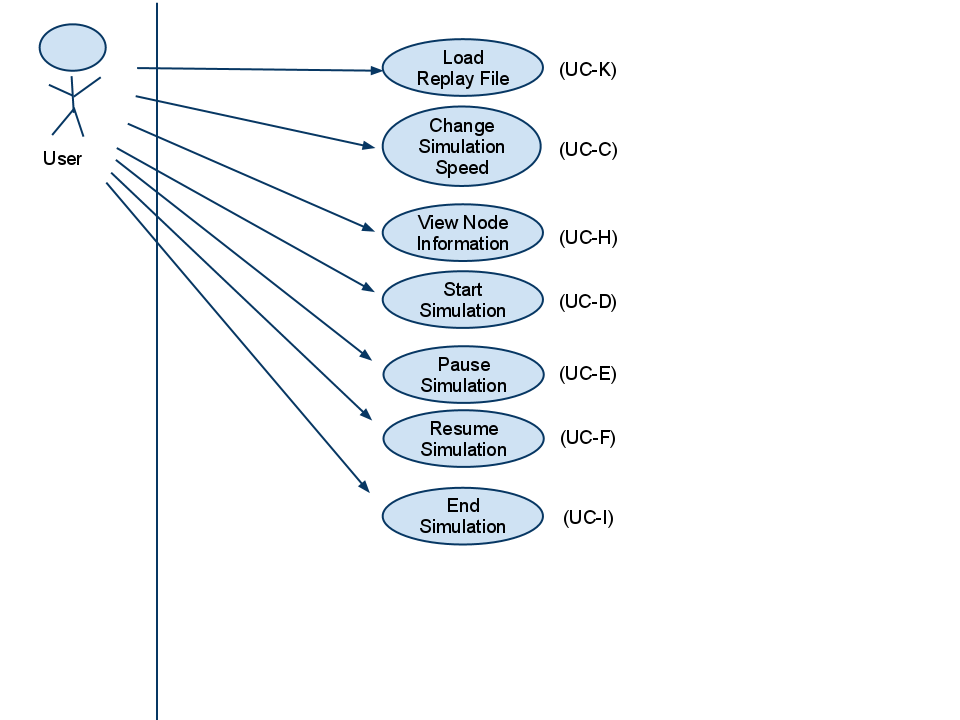
\includegraphics[height=150mm]{img/scenario2.png}
        \caption{Usage Scenario 2: Batch Mode}
        \label{fig:scen2}
\end{figure}

\subsection{Blended Mode Scenario}
The blended mode scenario represents an interaction that incorporates parts of the batch scenario and parts of the manual scenario.
 
The user begins by having DARS read in a log file using the import function. This causes the board to be populated with network nodes as they were at the beginning of the log file’s simulation. The user then elaborates upon this configuration at their discretion, continuing exactly as the manual scenario describes.

This scenario exposes the function points shown in figure \ref{fig:scen3} below.
\begin{figure}[H]
        \centering
	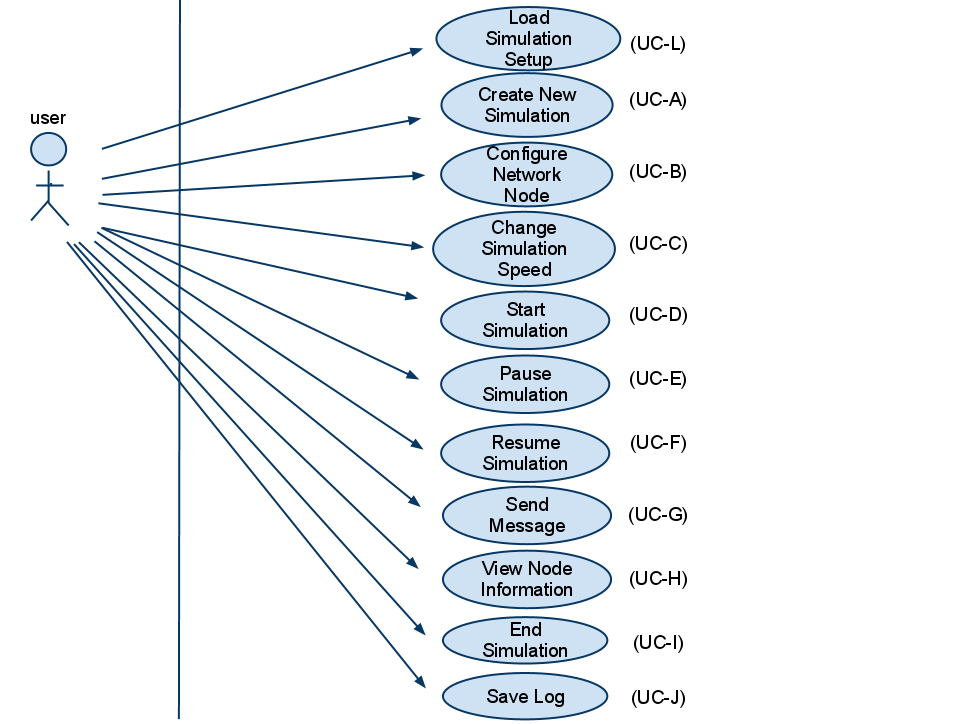
\includegraphics[height=150mm]{img/scenario3.png}
        \caption{Usage Scenario 3: Blended Mode}
        \label{fig:scen3}
\end{figure}

\section{Use Cases}

\subsection{Create New Simulation (UC-A)}
\subsubsection{Actors}
User.
\subsubsection{Description}
Create a new empty simulation.
\subsubsection{Trigger}
User selects File\ra New\ra $<$Protocol$>$
\subsubsection{Pre-conditions}

\begin{enumerate}
  \item User clicks the new option from the menu.
  \item User is presented with a dialog box to set network and protocol configuration items such as the bandwidth.
\end{enumerate}

\subsubsection{Post-conditions}

\begin{enumerate}
  \item User selects a valid protocol. 
  \item Log is cleared and a new log is created.
  \item New simulation entry is added to the log. 
\end{enumerate}

\subsubsection{Normal Flow}
\begin{enumerate}
  \item Routing protocol selected.
  \item Protocol and network parameters are set.
\end{enumerate}

\subsubsection{Alternative Flows}
None.
\subsubsection{Exceptions}

\begin{enumerate}
  \item  An error will be thrown if the log file can not be cleared.
  \item  An error will be thrown if a new log file can not be created.
\end{enumerate}

\subsubsection{Priority}
Critical.

\subsubsection{Frequency of Use}
Often.

\subsection{Configure Network Node (UC-B)}
\subsubsection{Actors}
User.
\subsubsection{Description}
Configure a network node.
\subsubsection{Trigger}
User Edits or Creates a Node.
\subsubsection{Pre-conditions}

\begin{enumerate}
  \item A simulation has been created.
  \item Simulation is not running.
\end{enumerate}

\subsubsection{Post-conditions}

\begin{enumerate}
  \item Node information is set.
  \item Log message is recorded.
\end{enumerate}

\subsubsection{Normal Flow}
\begin{enumerate}
  \item User Right clicks on a node and selects edit or user right clicks on the canvas and selects new.
  \item User is presented with dialog box to edit the node information.
  \item User enters the nodes information.
  \item User saves the node information and the dialog box closes.
\end{enumerate}

\subsubsection{Alternative Flows}

\begin{enumerate}
  \item User right clicks on a node and selects edit or user right clicks on the canvas and selects new.
  \item User cancels, no information is saved, and the dialog box closes.
\end{enumerate}

\subsubsection{Exceptions}

\begin{enumerate}
  \item  If a node parameter that is entered is invalid an error will be presented to the user.
\end{enumerate}

\subsubsection{Priority}
Critical.
\subsubsection{Frequency of Use}
Very often.

\subsection{Configure Simulation Speed (UC-C)}
\subsubsection{Actors}
User.
\subsubsection{Description}
Configure the speed of the simulation.

\subsubsection{Trigger}
User moves the speed slider.

\subsubsection{Pre-conditions}

\begin{enumerate}
  \item A simulation has been created.
  \item Simulation is not running.
\end{enumerate}

\subsubsection{Post-conditions}

\begin{enumerate}
  \item A new simulation speed is set.
\end{enumerate}

\subsubsection{Normal Flow}
\begin{enumerate}
  \item The user pauses the simulation, or simulation has not begun.
  \item The user moves the speed slider.
  \item The user resumes the simulation, or starts the simulation if not yet started.
\end{enumerate}

\subsubsection{Alternative Flows}
None.


\subsubsection{Exceptions}
None.

\subsubsection{Priority}
Moderate.

\subsubsection{Frequency of Use}
Infrequent.

\subsubsection{Notes and Issues}
As an enhancement in later versions of DARS the precondition of stopping the simulator could be lifted, but for simplicity this restriction will be enforced in the initial versions.

\subsection{Start Simulation (UC-D)}
\subsubsection{Actors}
User.
\subsubsection{Description}
Begin a Simulation.

\subsubsection{Trigger}
User clicks the ``play'' button from the GUI.

\subsubsection{Pre-conditions}

\begin{enumerate}
  \item The simulator has been presented with a valid simulation context via one of the following:
  \begin{itemize}
    \item The user has created a new simulation.
    \item The user has loaded a previous simulation.
    \item The user has paused a running simulation.
  \end{itemize}
\end{enumerate}

\subsubsection{Post-conditions}
\begin{enumerate}
  \item The simulation is running.
\end{enumerate}

\subsubsection{Normal Flow}
\begin{enumerate}
  \item User clicks on the ``play'' button and the simulation begins or resumes. 
\end{enumerate}

\subsubsection{Alternative Flows}
None.

\subsubsection{Exceptions}
None.

\subsubsection{Priority}
Critical.

\subsubsection{Frequency of Use}
Very Often.


\subsection{Pause Simulation (UC-E)}
\subsubsection{Actors}
User.

\subsubsection{Description}
Pause Simulation.

\subsubsection{Trigger}
User clicks ``pause'' button on the screen.

\subsubsection{Pre-conditions}

\begin{enumerate}
  \item Simulation already running.
\end{enumerate}

\subsubsection{Post-conditions}

\begin{enumerate}
  \item Simulation can be resumed from the same point where it was paused by clicking Play button on the screen.
\end{enumerate}

\subsubsection{Normal Flow}
\begin{enumerate}
  \item User clicks pause to pause the simulation.
\end{enumerate}

\subsubsection{Alternative Flows}
None.

\subsubsection{Exceptions}
None.


\subsubsection{Priority}
Moderate.

\subsubsection{Frequency of Use}
Infrequent.


\subsection{Resume Simulation (UC-F)}
\subsubsection{Actors}
User.
\subsubsection{Description}
Resume a simulation.
\subsubsection{Trigger}
User clicks the ``resume'' button.
\subsubsection{Pre-conditions}

\begin{enumerate}
  \item A simulation has been paused by the user.
\end{enumerate}

\subsubsection{Post-conditions}

\begin{enumerate}
  \item The simulation continues.
\end{enumerate}

\subsubsection{Normal Flow}
\begin{enumerate}
  \item User clicks the ``resume'' button to resume the simulation.
\end{enumerate}

\subsubsection{Alternative Flows}
None.

\subsubsection{Exceptions}
None.

\subsubsection{Priority}
Critical.

\subsubsection{Frequency of Use}
Infrequent.


\subsection{Send Message (UC-G)}
\subsubsection{Actors}
User.

\subsubsection{Description}
User sends a message from one node to another.

\subsubsection{Trigger}
User right clicks on a node and selects the ``Send Message'' option.
\subsubsection{Pre-conditions}

\begin{enumerate}
  \item Simulation is not running.
  \item The network has at least two nodes.
\end{enumerate}

\subsubsection{Post-conditions}

\begin{enumerate}
  \item Message is introduced into the network.
  \item Message send action is logged.
\end{enumerate}

\subsubsection{Normal Flow}
\begin{enumerate}
  \item User right clicks on a node (Sender).
  \item User is presented with a send message dialog box.
  \item User selects a Destination Node from a drop down box.
  \item User enters message.  
  \item User selects send message.
\end{enumerate}

\subsubsection{Alternative Flows}
None.

\subsubsection{Exceptions}
None.

\subsubsection{Priority}
Critical.

\subsubsection{Frequency of Use}
Often.

\subsubsection{Notes and Issues}
As an enhancement in later versions of DARS the precondition of stopping the simulator could be lifted, but for simplicity this restriction will be enforced in the initial versions.


\subsection{View Node Information (UC-H)}
\subsubsection{Actors}
User.
\subsubsection{Description}
Display a node’s information.
\subsubsection{Trigger}
Select a node.
\subsubsection{Pre-conditions}

\begin{enumerate}
  \item  At least one node exists.
\end{enumerate}

\subsubsection{Post-conditions}

\begin{enumerate}
  \item The selected node’s information is displayed in the node information panel on the right side of the DARS window.
\end{enumerate}

\subsubsection{Normal Flow}
\begin{enumerate}
  \item User left clicks on a node.
  \item User observes node information displayed in the node information panel. 
\end{enumerate}

\subsubsection{Alternative Flows}

\begin{enumerate}
  \item User selects or searches for a node from the drop down list at the top of the node information panel.
  \item  User observes node information displayed in the node information panel.
\end{enumerate}


\subsubsection{Exceptions}
None.

\subsubsection{Priority}
Critical.

\subsubsection{Frequency of Use}
Very often.

\subsubsection{Notes and Issues}
This is the primary means for a user to look at a nodes routing table.  With out this it will be decidedly harder to see the differences between the various protocols.

\subsection{End Simulation (UC-I)}
\subsubsection{Actors}
User.
\subsubsection{Description}
End the currently running simulation.
\subsubsection{Trigger}
User clicks the ``Stop'' button.
\subsubsection{Pre-conditions}

\begin{enumerate}
  \item Simulation has been started.
\end{enumerate}

\subsubsection{Post-conditions}

\begin{enumerate}
  \item Simulation ends.
\end{enumerate}

\subsubsection{Normal Flow}
\begin{enumerate}
  \item User selects the ``Stop'' button.
\end{enumerate}

\subsubsection{Alternative Flows}
None.

\subsubsection{Exceptions}
None.

\subsubsection{Priority}
High.

\subsubsection{Frequency of Use}
Infrequent.


\subsection{Save Log (UC-J)}
\subsubsection{Actors}
User.
\subsubsection{Description}
User saves replay log to a file of their choosing.
\subsubsection{Trigger}
User clicks File \ra Save. 
\subsubsection{Pre-conditions}

\begin{enumerate}
  \item A simulation has already been created.
  \item The simulation is not running.
\end{enumerate}

\subsubsection{Post-conditions}
 
\begin{enumerate}
  \item A replay log is saved to a user defined location.
\end{enumerate}

\subsubsection{Normal Flow}
\begin{enumerate}
  \item User clicks File \ra Save. 
  \item User is presented with a save file dialog box.
  \item User enters the file name and location for the replay log.
  \item User saves the file.
\end{enumerate}

\subsubsection{Alternative Flows}

\begin{enumerate}
  \item User clicks File \ra Save.
  \item User is presented with a save file dialog box.
  \item User Cancels the action.
\end{enumerate}

\subsubsection{Exceptions}

\begin{enumerate}
  \item  User is unable to save the log file to the filesystem due to a write error.
\end{enumerate}

\subsubsection{Priority}
High.

\subsubsection{Frequency of Use}
Infrequent.


\subsection{Load Replay File (UC-K)}
\subsubsection{Actors}
User.
\subsubsection{Description}
Load replay file.
\subsubsection{Trigger}
User clicks on File \ra Import \ra Replay.
\subsubsection{Pre-conditions}

\begin{enumerate}
  \item A simulation file exists.
\end{enumerate}

\subsubsection{Post-conditions}

\begin{enumerate}
  \item  Previous simulation run is replayed.     
\end{enumerate}

\subsubsection{Normal Flow}
\begin{enumerate}
  \item User clicks on File \ra Import \ra Replay.
  \item  User is presented with a replay file dialog box.
  \item User loads the replay file in the replay file dialog box.
  \item User clicks replay in the replay dialog box.
\end{enumerate}

\subsubsection{Alternative Flows}

\begin{enumerate}
  \item User clicks on File \ra Import \ra Replay.
  \item User is presented with a replay file dialog box.
  \item User cancels the action.
\end{enumerate} 

\subsubsection{Exceptions}

\subsubsection{Priority}
High.

\subsubsection{Frequency of Use}
Infrequent.


\subsection{Import Setup (UC-L)}
\subsubsection{Actors}
User.
\subsubsection{Description}
The network node arrangement of a previous run is imported into the simulation.
\subsubsection{Trigger}
  User clicks on File \ra Import \ra Setup.
\subsubsection{Pre-conditions}

\begin{enumerate}
  \item A simulation file must have been previously saved.
\end{enumerate}

\subsubsection{Post-conditions}

\begin{enumerate}
  \item The setup of a previously run simulation is loaded into the current simulation.
\end{enumerate}

\subsubsection{Normal Flow}
\begin{enumerate}
  \item User clicks on File \ra Import \ra Setup.
  \item The user is presented with the load replay setup dialog.
  \item The user selects a file from the load replay setup dialog.
  \item The previous configuration is loaded into the current simulation window.
  \item The user can run the replay as if they had manually entered all of the loaded information.
\end{enumerate}

\subsubsection{Alternative Flows}

\begin{enumerate}
  \item The user is prompted with the load replay setup dialog.
  \item The user cancels the operation.
\end{enumerate}

\subsubsection{Exceptions}
None.

\subsubsection{Priority}
High.

\subsubsection{Frequency of Use}
Infrequent.

\end{document}
